% ============================ Enrico Ribiani 16-03-2021 ====================================================================
% Base per i documenti  
\documentclass[12pt]{article}
% ------------ pacchetti necessari ----------------
\usepackage[a4paper, total={6in, 8in},margin=1in]{geometry} % formattazione decente della pagina
\usepackage{graphicx}                            % need for figure
\usepackage{amsmath}
\usepackage{amsfonts}                            % if you want the fonts
\usepackage{amssymb}                             % if you want extra symbols
\usepackage{graphicx}  
\renewcommand{\figurename}{Figura}  
\renewcommand{\contentsname}{Indice}                        % need for figures
\usepackage{mathptmx}
\usepackage{float}                               % serve per mettere tabelle e immagini dove si vuole 
\usepackage[utf8]{inputenc}
\usepackage{textcomp}
\usepackage[hang,flushmargin,bottom]{footmisc}   % footnote format
\usepackage{fancyhdr, lastpage}
\usepackage{titlesec}
\usepackage[table,dvipsnames]{xcolor}
%\pagestyle{fancy}
%\renewcommand{\headrulewidth}{0pt}
%\renewcommand*\contentsname{Indice}
\titleformat{\section}{\normalsize\bfseries}{\thesection.}{1em}{}	% required for heading numbering style
\titleformat*{\section}{\Large\bfseries}
\titleformat*{\subsection}{\large\bfseries}
%\usepackage{siunitx}
%\usepackage{tikz}
\usepackage{circuitikz}
\usepackage{multicol}
%\usepackage[siunitx]{circuitikz}
\usepackage{multirow}
\usepackage{tikz}
\usepackage{amsmath}
\usetikzlibrary{angles,quotes}
\usepackage{placeins}

\usepackage{wasysym}
%===================links=================
\usepackage{hyperref}
\hypersetup{
    colorlinks=true,
    linkcolor=darkgray,
    filecolor=Green,      
    urlcolor=Cyan,
    pdftitle={SAMPLE},
    pdfpagemode=FullScreen,
    }
%===================inizio pagina del titolo=================
\begin{document}
\begin{titlepage}
	\begin{center}
		% ------------------ inizio immagine logo ----------
		\begin{figure}
			\centering
			
\includegraphics[scale=1.3]{/home/r1bbi/Documenti/latec/logo.png}

		\end{figure}
		% ------------------ fine immagine logo ----------
		% ------------------ fine immagine logo ----------
		-------------------------------------------------------------------------------------\\
		\vspace{2\baselineskip}
		\large Prova n°7
		\hfill
		\large $5^a$   AUB\\
		\begin{flushleft}
			\large Enrico Ribiani\\
			\large Daniel Graziadei\\
			\large Gruppo 11\\
		\end{flushleft}


		\vfill

		\Huge{\textbf{Ponte H}}\\
		\vfill
		\vfill
		\large{30-3-2023}
	\end{center}
	%=============== fine pagina titolo ===============
\end{titlepage}
\thispagestyle{empty}
\tableofcontents
\newpage
\setcounter{page}{1}
\vskip 1cm
\section{Scopo}
Azionamento di un motore DC tramite Arduino UNO

\section{Schema}

\begin{figure}[!h]
	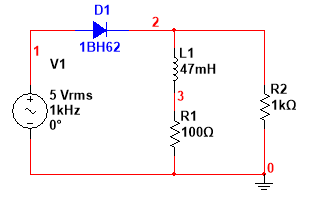
\includegraphics[scale=0.7]{schema.PNG}
\end{figure}
\href{https://www.google.com/url?sa=i&url=https%3A%2F%2Flogicaprogrammabile.it%2Fpilotare-motore-dc-tramite-ponte-h%2F&psig=AOvVaw3HWeGK16jnlvwXhPIfXFen&ust=1681318364866000&source=images&cd=vfe&ved=0CBMQjhxqFwoTCMipiJelov4CFQAAAAAdAAAAABAD}{fonte}

\section{Materiale e Strumenti}
	\begin{itemize}
		\item Generatore DC 5V
		\item 2x BJT pnp BC327
		\item 2x BJT npn BC333
		\item 4x diodi 
		\item 4x resistore 1k$\Omega$
		\item Arduino UNO
		\item Motore DC
	\end{itemize}

\section{Contenuti Teorici}
Per far girare il motore in entrambe le direzioni ci sarà bisogno di alimentarlo tramite un ponte H e controllare
i transistor BJT due a due tramite un arduino uno.\\
Per combinare il circuito di potenza con la parte di controllo viene usato un circuito chiamato ponte H
costituito da due transistor npn, e due pnp.\\
I diodi vengono alimentati due a due, un pnp con un npn e alimentano il motore accendendosi in contrapposizione.\\
Per fare ciò bisogna posizionare i pnp in "basso" e gli npn in "alto", così in base a quale lato è alimentato  
la correntepuò attraversare il motore in entrambi i lati.\\
L'arduino ha il compito ciclicamente di accendere due a due i transistor alernando la marcia.\\

\section{Raccolta Dati}
\begin{figure}[H]
   
    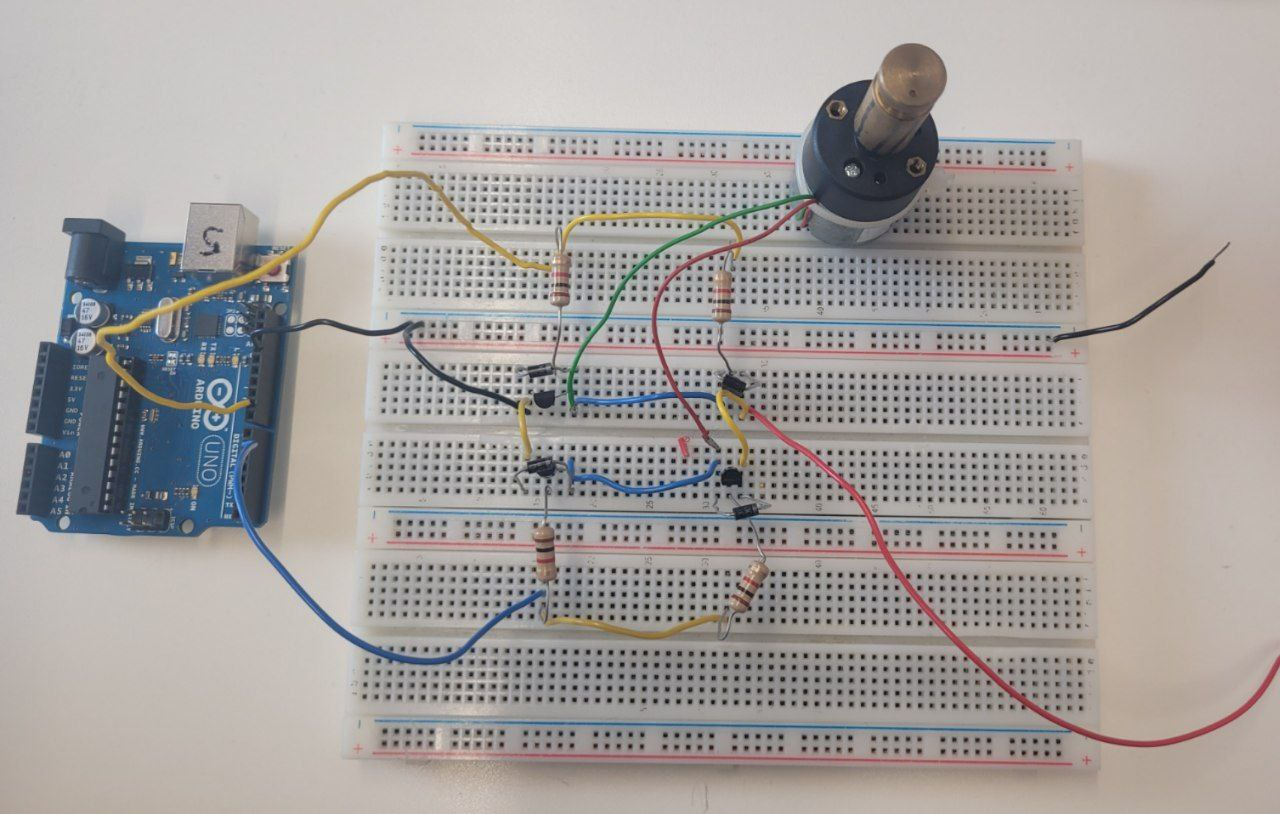
\includegraphics[scale=0.3]{montaggio.jpg}
\end{figure}



\section{Analisi critica dei risultati e conclusioni}
Montato il circuito e scritto il breve codice necessario a far funzionare il motore, abbiamo alimentato il circuito
e il motore ha iniziato a girare prima in un verso e poi in un altro per il tempo da noi stabilito tramite il 
programma.
Abbiamo avuto la prova che ponte H è stato montato correttamente.\\
\end{document}
